\documentclass[11pt]{article}

\usepackage[margin=1in]{geometry}
\usepackage[T1]{fontenc}
\usepackage[utf8]{inputenc}
\usepackage{lmodern}
\input{glyphtounicode}
\pdfgentounicode=1
\usepackage{graphicx}
\usepackage{booktabs}
\usepackage{array}
\usepackage{amsmath}
\usepackage{placeins}
\usepackage{hyperref}
\usepackage[protrusion=true,expansion=false]{microtype}
\emergencystretch=2em

\title{State-Transfer Protocols for Multilingual Multi-Agent Handoff}
\author{Jordy Hernandez Cruzado\\Hijos Del Sol Research\\\texttt{hernandezcruzadojordy@gmail.com}}
\date{}

\begin{document}
\maketitle

\begin{abstract}
Large language model agents increasingly need to continue work after context truncation, provider failure, model substitution, or handoff to another agent. This paper studies compact prompt formats as \emph{state-transfer protocols}: reusable communication formats intended to preserve operational state rather than merely reduce token count. We evaluate four modes---\texttt{natural}, \texttt{compressed}, \texttt{hybrid\_min}, and \texttt{hybrid\_state}---across multilingual, multi-model, judge-based, and real-agent settings. EXP05 provides a broad discovery study over Spanish, English, and Chinese tasks with multiple generator families. EXP06 is a controlled follow-up comparing \texttt{compressed} against \texttt{hybrid\_state}, including language/variant ablations and three-judge calibration. EXP07 and EXP08 move beyond LLM-as-judge evaluation by testing real-agent handoff in LangGraph/OpenFang-style surfaces with objective continuation metrics. EXP13--EXP16 extend this into controlled repository maintenance, long-horizon public-page editing, and model-specific protocol adaptation. Across these experiments, \texttt{compressed} is the strongest general baseline, while \texttt{hybrid\_state} improves judge-scored state preservation in paired comparisons but does not win global quality or real-agent operational performance. We argue that prompt compression should be reframed as protocol design: compact formats should be selected by target function, such as semantic quality, state preservation, continuity, cost, or interface reliability.
\end{abstract}

\section{Introduction}
Agentic LLM systems are often interrupted. Context windows end, workers change, provider quotas fail, and downstream agents need a compact representation of what happened. A common response is to summarize more context in natural language. That is useful, but it is not the same as preserving operational state. Variables, constraints, unfinished subtasks, plans, and forbidden claims can disappear even when the summary sounds fluent.

This paper asks whether compact prompt formats can be treated as \emph{state-transfer protocols}. The question is not only whether a prompt can be shorter, but whether it can carry the right state for another model, language, or agent surface to continue the task. This distinction matters because the best format for global quality may differ from the best format for handoff continuity.

The main claim is deliberately narrow. \texttt{compressed} is a robust universal baseline. \texttt{hybrid\_state} is not a global winner, but it is a specialized protocol that improves state preservation in judge-scored paired designs. In real-agent settings, the advantage becomes conditional: objective validators show that \texttt{compressed} often remains stronger, while \texttt{hybrid\_state} can help selected constraint/plan strata.

\section{Related Work}
This work sits between prompt compression, agent memory, tool-use evaluation, and LLM-as-judge methodology. Prompting work such as chain-of-thought shows that format changes can alter model behavior, but the goal here is not to elicit longer reasoning; it is to transfer compact operational state across handoffs. Prompt-compression work such as LLMLingua shows that inputs can often be shortened without proportional quality loss, but our focus is not only token reduction: it is whether compact formats preserve variables, constraints, and next actions. ReAct-style systems connect language models to action traces and tools, making state representation a practical interface problem rather than only a prompt-design problem. Agent-memory systems such as Generative Agents highlight the value of persistent state, while long-context studies show that simply storing more text does not guarantee retrieval or use of the right information. Finally, LLM evaluation surveys motivate caution around judge-scored results; for this reason, EXP07 and EXP08 add objective continuation metrics and treat EXP09--EXP16 as interface and repository validations rather than broad agent benchmarks.

\section{Protocols}
We evaluate four communication modes. Table~\ref{tab:protocol_examples} shows the same handoff task rendered in each style.

\begin{table}[h]
\centering
\scriptsize
\begin{tabular}{p{0.18\linewidth}p{0.74\linewidth}}
\toprule
Mode & Example handoff for: ``continue EXP06 analysis without claiming global win''\\
\midrule
\texttt{natural} & Continue the EXP06 analysis. The current result is that \texttt{compressed} remains stronger on global quality, while \texttt{hybrid\_state} improves state preservation. Do not claim that \texttt{hybrid\_state} wins overall. Next, report paired deltas and limitations.\\
\texttt{compressed} & goal=EXP06 report; state=compressed wins Q, hybrid\_state wins state; forbid=``hybrid\_state global winner''; evidence=paired deltas; next=write result + limitation; risk=overclaim.\\
\texttt{hybrid\_min} & g=EXP06; st=comp>Q, hs>state; !claim=hs global win; e=paired deltas; n=report+limit; r=overclaim.\\
\texttt{hybrid\_state} & \texttt{HYBRID\_STATE\{G:EXP06; VAR:[base=compressed, cand=hybrid\_state]; C:[no global-win claim]; E:[Q lower, state higher]; PLAN:[paired deltas, language ablation, limits]; NEXT:bounded result\}}\\
\bottomrule
\end{tabular}
\caption{Concrete protocol examples. The distinction is not only brevity: \texttt{hybrid\_state} makes operational variables and constraints explicit.}
\label{tab:protocol_examples}
\end{table}

\section{Experimental Design}
\textbf{EXP05} is a broad discovery experiment. It evaluates 15 task templates across Spanish (ES), English (EN), and Chinese (ZH), four protocol modes, two repetitions, and five generator families: Grok 4.20 Non-Reasoning, Gemini 3.1 Pro Preview, Llama 4 Maverick, Qwen3-Next-80B, and GLM 5. Judges return strict JSON metrics including semantic fidelity, utility, state preservation, operational continuity, handoff quality, compactness, ambiguity, and information loss.

\textbf{EXP06} is a controlled follow-up. It compares \texttt{compressed} and \texttt{hybrid\_state} under paired cells, adds language/variant ablations (ES, EN, ZH, ZH\_PINYIN, ES\_LITERAL, EN\_LITERAL), and evaluates valid generations with three judge routes: Gemini 3.5 Flash, Azure GPT 5.4 High, and Grok 4.20 Reasoning.

\textbf{EXP07} and \textbf{EXP08} test real-agent handoff. They use LangGraph/OpenFang-style execution with objective metrics: variable recovery, subtask completion, plan continuity, constraint retention, handoff success, and state-error count. EXP07 contains 270 cleaned executions. EXP08 scales to 900 operational executions and reports both an operational-complete view and a strict JSON-valid view.

\textbf{EXP09--EXP16} are not treated as central evidence for global protocol superiority in this paper. They are interface-validation and repository-maintenance studies. EXP10--EXP12 validate public page/repo maintenance; EXP13 is the principal controlled multi-agent scientific-repository benchmark. EXP14 and EXP15 extend the setting to repeated repo/page maintenance and visual/responsive scale-up. EXP16 tests model-specific protocol adaptations and records a provider-restriction event that interrupted the full run. Their results are best read as engineering and systems evidence about action schemas, parsers, validators, checksums, role-conditioned handoff, model-route compatibility, provider quotas, and reasoning-budget behavior.

\section{Results}
\begin{table}[t]
\centering
\scriptsize
\begin{tabular}{p{0.13\linewidth}p{0.26\linewidth}p{0.22\linewidth}p{0.30\linewidth}}
\toprule
Exp. & Role & Key result & Interpretation\\
\midrule
EXP05 & Broad multilingual discovery & \texttt{compressed} strongest overall; \texttt{hybrid\_state} improves state preservation by $+0.133$ vs. \texttt{compressed} & State preservation can diverge from global quality.\\
EXP06 & Controlled paired follow-up & \texttt{hybrid\_state} loses quality ($-0.208$) but gains state preservation ($+0.066$) & Confirms specialization, rejects global-win claim.\\
EXP07 & Real-agent objective handoff & \texttt{compressed} leads variable recovery and plan continuity; \texttt{hybrid\_state} only slightly higher on constraints & Judge-state gains do not automatically transfer to operational metrics.\\
EXP08 & Real-agent scale-up & 900 operational executions; strict JSON-valid view exposes 76 blank-output failures in GPT 5.4 High & Protocol behavior depends on parsers, schemas, and serving route behavior.\\
EXP13 & Scientific-repo benchmark & 126/128 real model cells; \texttt{compressed}=64/64, \texttt{hybrid\_state}=62/64 & \texttt{compressed} was more operationally robust; \texttt{hybrid\_state} exposed longer-task contract fragility.\\
EXP15-B & Visual/responsive scale-up & 1204/2000 latest cells succeeded; Grok Reasoning improved over Non-Reasoning by 13.75 points but remained fragile & Later repo/page tasks are best interpreted as contract/interface compatibility tests, not visual-design leaderboards.\\
EXP16 & Model-specific adaptation & 320/421 latest cells succeeded before provider restriction; \texttt{model\_adapted} was strongest for Qwen and Gemini 3.5 Flash in round 1 & Model-specific prompts help some routes, but platform failures must be separated from model/protocol failures.\\
\bottomrule
\end{tabular}
\caption{Compact summary of the main evidence used in this short paper. EXP09--EXP16 support interface and repository-validity claims, not broad claims that one protocol solves general agent work.}
\label{tab:key_results}
\end{table}

\subsection{EXP05: Broad Discovery}
Figure~\ref{fig:exp05_modes} summarizes EXP05. \texttt{compressed} is the strongest global baseline. \texttt{hybrid\_state} is close on global quality and improves state preservation in paired analysis, while \texttt{hybrid\_min} preserves compactness but loses quality.

\begin{figure}[h]
\centering
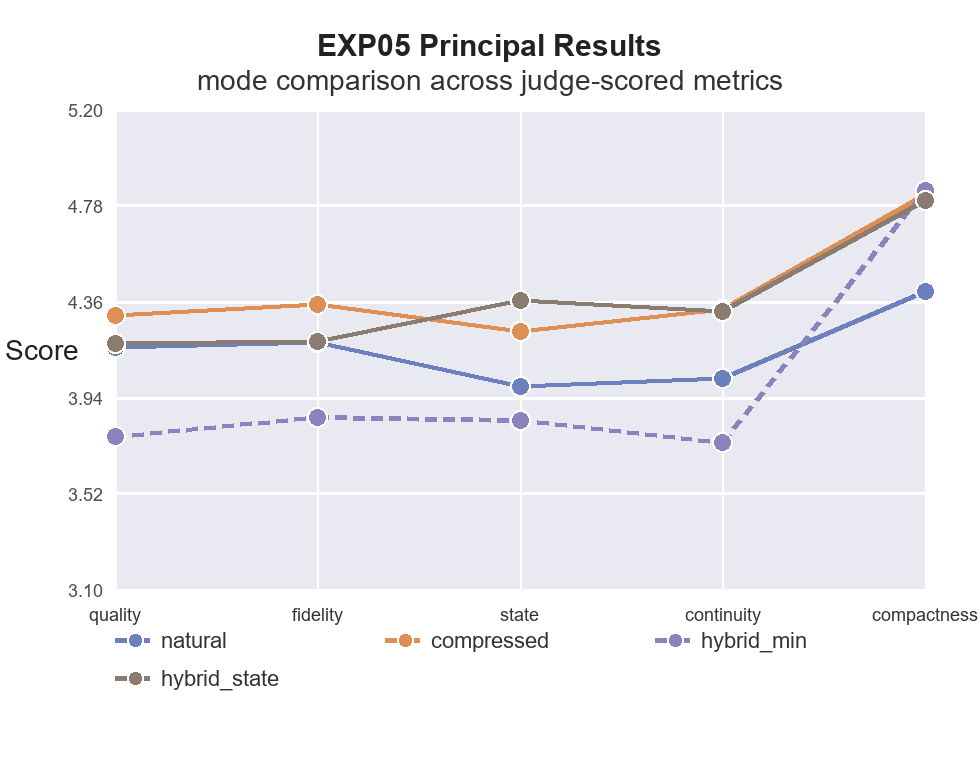
\includegraphics[width=0.82\linewidth]{figures/fig_exp05_modes.png}
\caption{EXP05 principal results by protocol mode. The curve shape is the key result: compactness alone is not enough, and state preservation separates \texttt{hybrid\_state} from \texttt{hybrid\_min}.}
\label{fig:exp05_modes}
\end{figure}

The paired comparison against \texttt{compressed} shows the tradeoff directly. \texttt{hybrid\_state} improves state preservation by $+0.133$ with 95\% CI $[+0.025,+0.240]$, while losing global quality by $-0.108$ with 95\% CI $[-0.203,-0.012]$. Operational continuity is effectively tied.

\subsection{EXP06: Controlled Follow-Up}
EXP06 confirms the state-preservation interpretation but weakens any global-win interpretation. Figure~\ref{fig:exp06_modes} shows that \texttt{compressed} remains stronger on quality, fidelity, compactness, and lower ambiguity/information loss, while \texttt{hybrid\_state} is higher on state preservation.

\begin{figure}[h]
\centering
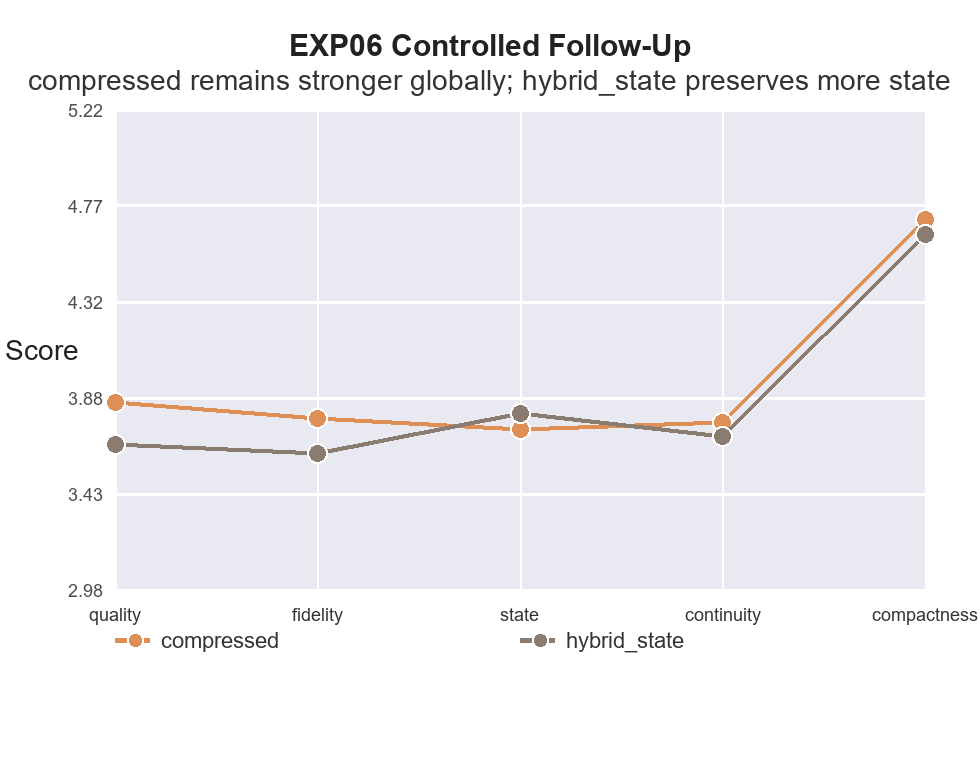
\includegraphics[width=0.82\linewidth]{figures/fig_exp06_modes.png}
\caption{EXP06 controlled follow-up. \texttt{hybrid\_state} is a state-oriented specialization, not a universal quality improvement.}
\label{fig:exp06_modes}
\end{figure}

Overall paired quality favors \texttt{compressed}. The observed \texttt{hybrid\_state} minus \texttt{compressed} quality delta is -0.208, with 95\% CI [-0.239, -0.177]. State preservation moves in the opposite direction: +0.066, with 95\% CI [+0.032, +0.100]. This is the central controlled result.

Figure~\ref{fig:exp06_lang} shows quality deltas by language/variant. Native ZH remains more favorable than ZH\_PINYIN, suggesting that representation matters, but this should be treated as a promising signal rather than a causal tokenization proof.

\begin{figure}[h]
\centering
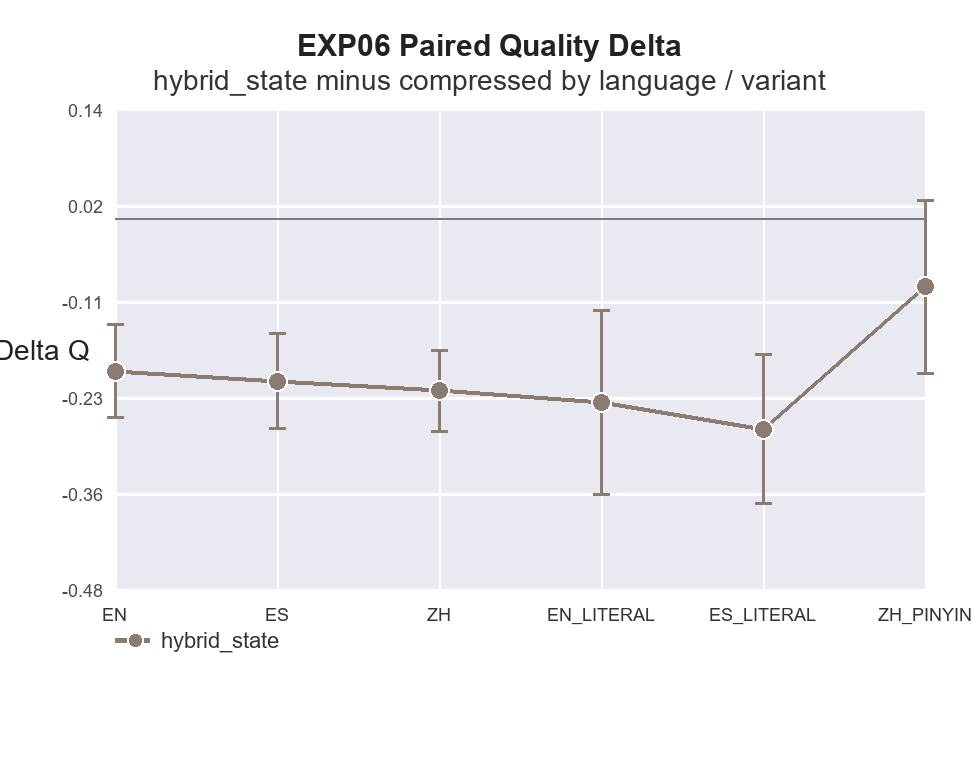
\includegraphics[width=0.82\linewidth]{figures/fig_exp06_language_delta.png}
\caption{EXP06 paired quality delta for \texttt{hybrid\_state} minus \texttt{compressed}. Negative values mean \texttt{compressed} remains stronger on global quality.}
\label{fig:exp06_lang}
\end{figure}

\subsection{EXP07/EXP08: Real-Agent Objective Metrics}
EXP07 and EXP08 reduce dependence on LLM judges by scoring continuation behavior directly. Figure~\ref{fig:real_agent_objective} shows the compact objective-metric view.

\texttt{compressed} leads variable recovery and plan continuity. \texttt{hybrid\_state} is only slightly higher on constraint retention, and does not dominate globally.

EXP08 scales the setting to 900 operational executions. The operational-complete view again favors \texttt{compressed} globally. The strict JSON-valid view reveals a separate model/serving failure mode: Azure GPT 5.4 High produced 76 blank-output cells under strict JSON scoring, concentrated more heavily in \texttt{hybrid\_state}. This supports a systems interpretation: protocol performance depends on parser contracts, model route behavior, and output-budget settings.

\begin{figure}[h]
\centering
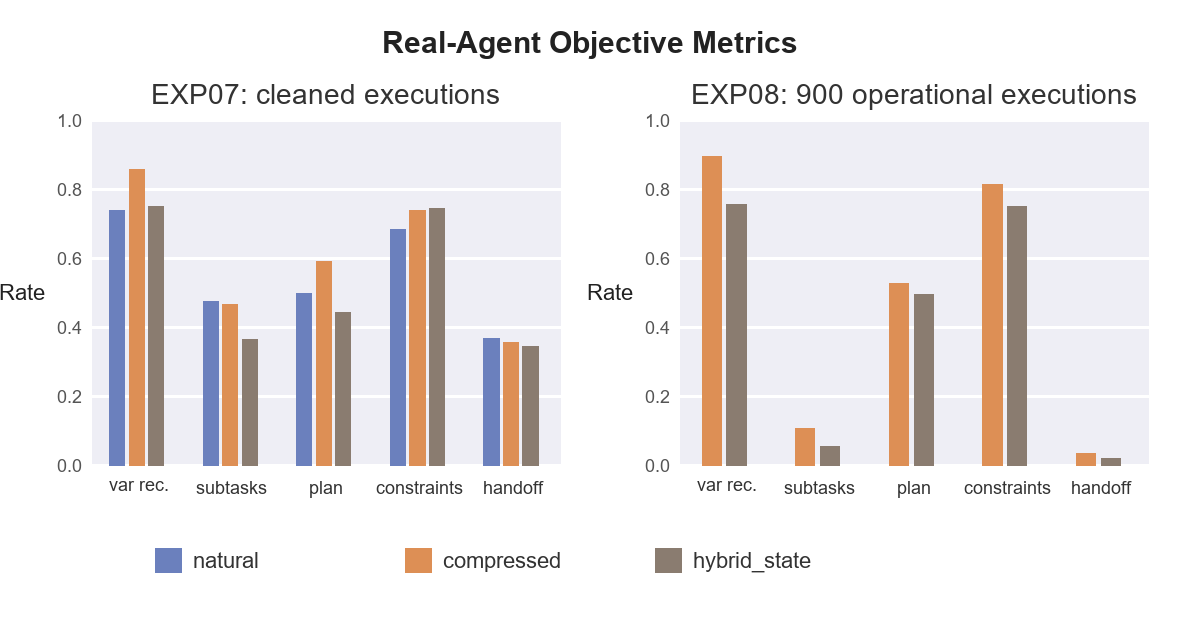
\includegraphics[width=0.98\linewidth]{figures/fig_exp07_exp08_objective_compact.png}
\caption{EXP07/EXP08 real-agent objective metrics with rate axes fixed to $[0,1]$. The compact view reduces reliance on LLM judges while showing that \texttt{compressed} remains the stronger operational baseline in these settings.}
\label{fig:real_agent_objective}
\end{figure}
\FloatBarrier

\subsection{EXP14/EXP15: Long-Horizon Repository Maintenance}
The later repository experiments stress repeated editing rather than isolated handoff. EXP14 completes 307/320 real-model latest cells and 55/64 complete chains. EXP15 freezes 818/900 successful latest cells and 141/180 complete chains. EXP15-B increases the visual/responsive scale to 2000 latest cells and 10-round chains, yielding 1204 successful latest cells and 71/200 complete chains. Figure~\ref{fig:exp15b_model} shows that the main signal is not aesthetic quality: the visual proxy saturated among successful pages. The discriminative result is contract compatibility. Grok 4.20 Reasoning improves over Grok 4.20 Non-Reasoning by 13.75 percentage points, but both routes remain much more fragile than Gemini 3.5 Flash, GLM 5, and Qwen3-Next-80B under the current parser/tool contract.

\begin{figure}[h]
\centering
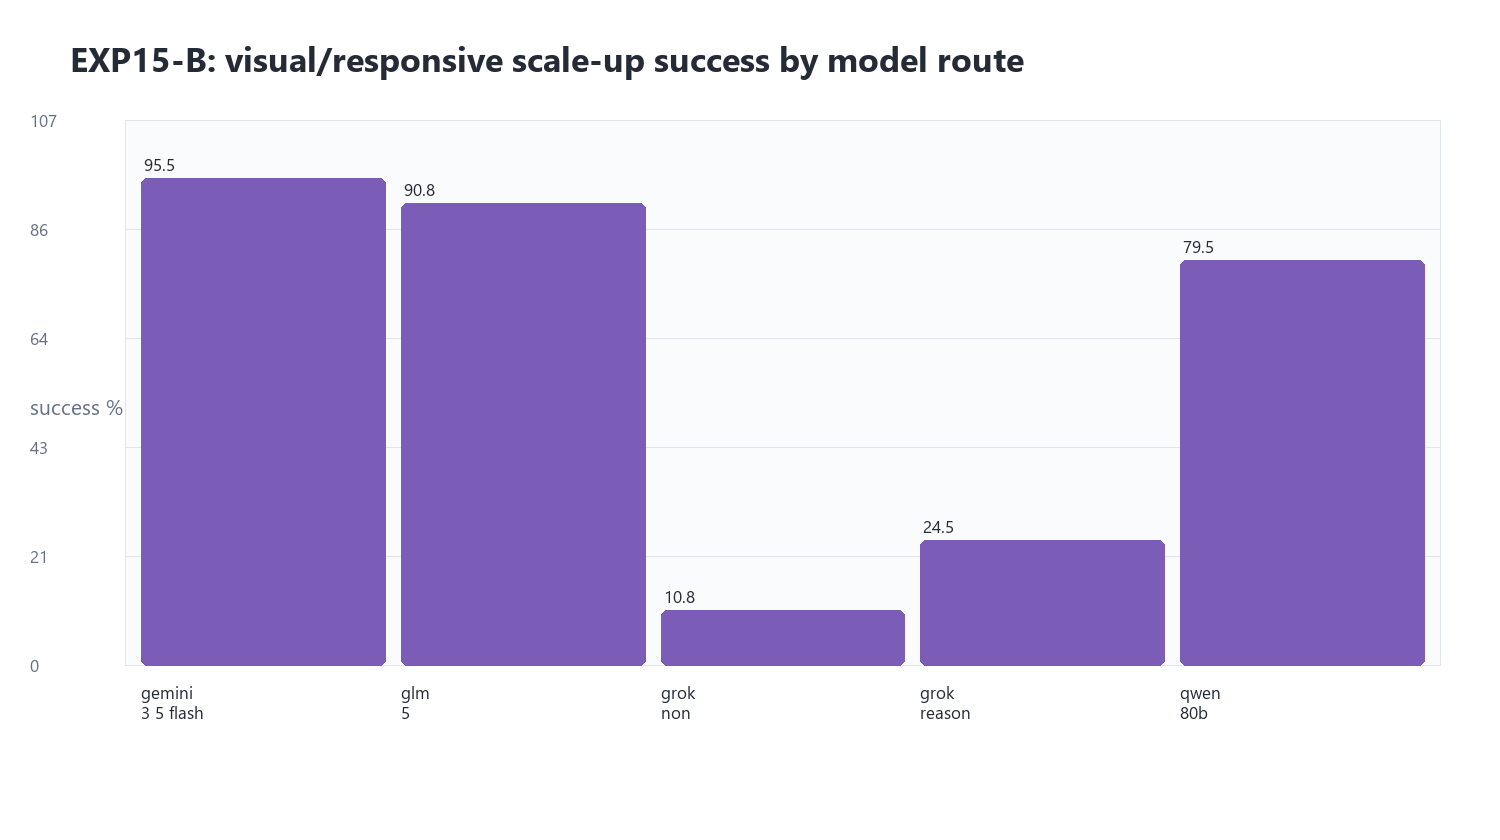
\includegraphics[width=0.9\linewidth]{figures/fig_exp15b_success_by_model.png}
\caption{EXP15-B success by model route. This figure should be read as operational compatibility under a strict repo/page editing contract, not as a general model-quality ranking.}
\label{fig:exp15b_model}
\end{figure}
\FloatBarrier

\subsection{EXP16: Model-Specific Protocol Adaptation}
EXP16 asks whether a frozen general protocol should be adapted to model route. The available round-1 data contain 421 latest cells, of which 320 are successful or repaired-success cells. The run was interrupted by a Google Cloud/Vertex provider restriction on 2026-05-30, so EXP16 is reported as a partial systems result rather than a complete benchmark.

The useful signal is route-specific. GLM 5 completed 96/96 round-1 cells. Qwen3-Next-80B succeeded on 88/96 cells, with \texttt{model\_adapted}=32/32. Gemini 3.5 Flash succeeded on 83/96 cells, with \texttt{model\_adapted}=30/32, higher than \texttt{compressed\_general}=28/32 and \texttt{hybrid\_state\_general}=25/32. Grok 4.20 Reasoning was confounded by quota, authentication, and provider-suspension errors. EXP16-B therefore tested five Grok-specific contracts; \texttt{grok\_v5\_two\_phase\_hidden} reached 19/32 and \texttt{grok\_v4\_schema\_echo} reached 18/32, while v1--v3 stayed below 6/32. Most remaining Grok failures were infrastructure errors, not semantic or JSON-contract failures.

EXP16 strengthens the systems claim rather than the global protocol claim: model-specific protocols can improve contract fit for some routes, but provider stability, authentication, quota windows, and suspension events must be modeled as first-class experimental outcomes.

\FloatBarrier

\section{Discussion}
The results support a target-function view of compact protocols. If the goal is broad semantic quality and robustness, \texttt{compressed} is the safest baseline. If the goal is explicit state preservation under judge-scored handoff, \texttt{hybrid\_state} is a useful specialization. If the goal is real-agent execution, the protocol alone is insufficient: schemas, parsers, validators, and model serving behavior become part of the experimental surface.

The ZH signal is interesting but not settled. EXP05 shows strong ZH performance, and EXP06 shows that native ZH is more favorable than ZH\_PINYIN. This supports a representation hypothesis, but does not isolate tokenizer mechanics from training distribution, script familiarity, or provider routing.

EXP09--EXP16 are best treated as interface and repository lessons. EXP09 and EXP10 have saturated final success rates, so their repaired failures are more informative than their aggregate success: schema mismatch, parser contract failures, checksum hallucination, missing tool names, and thinking-budget/output behavior. EXP13 is more discriminative: \texttt{compressed} completed 64/64 real cells, while \texttt{hybrid\_state} completed 62/64 and retained two final failures, one JSON-contract failure and one no-change failure. EXP15-B and EXP16 make the next issue clearer: the same model can look much stronger or weaker depending on how well its output style fits the tool contract and provider route. These are not distractions; they are exactly the kinds of failures that determine whether a state-transfer protocol survives contact with real tools and repo-maintenance tasks.

\section{Limitations}
The experiments are systems-oriented and provider-dependent. Model names, routes, quotas, and serving behavior are time-sensitive. EXP05 is broad and exploratory. EXP06 is better controlled but still relies on LLM judges. EXP07 and EXP08 add objective metrics, but their framework surfaces are not interchangeable. EXP14 and EXP15 add longer repo/page chains, but their validators still under-measure subjective visual quality. EXP16 was interrupted by provider restriction, and its platform errors are reported separately rather than scored as model/protocol failures. The quality index is descriptive rather than psychometrically validated. Strong claims should therefore rely on individual metrics and paired contrasts, especially state preservation and operational continuity.

The statistical analysis uses paired deltas and confidence intervals. A stronger venue submission should add clustered bootstrap or mixed-effect models over task, language, generator, judge, and repetition. This is especially important because the design contains multiple comparisons and correlated cells.

\section{Conclusion}
Prompt compression should be reframed as state-transfer protocol design. Across EXP05--EXP08, \texttt{compressed} is the robust universal baseline. \texttt{hybrid\_state} is a narrower state-oriented protocol: it improves judge-scored state preservation but does not win global quality or real-agent operational metrics. EXP13--EXP16 extend the lesson into repository maintenance: the protocol, model route, parser, validator, and provider surface form one coupled system. The most useful outcome is therefore not a single winning prompt style, but a clearer experimental vocabulary for evaluating agent handoff: semantic quality, state preservation, continuity, compactness, objective recovery, interface reliability, and platform robustness.

\FloatBarrier
\section*{Data and Code Availability}
All central claims in this short paper are supported by the long technical report and reproducibility package. The public repository is available at \url{https://github.com/DaosPath/state-transfer-protocols} and the archived release is available through Zenodo at \url{https://doi.org/10.5281/zenodo.20425831}. The technical report contains the extended methodology, experiment history, cost notes, error analysis, and appendices. The reproducibility repository contains prompts, task banks, validators, schemas, cleaned latest-cell datasets, repaired-error logs, analysis scripts, freeze manifests, and checksum manifests. Public release excludes API keys, credential files, private provider logs, and unredacted local paths.

\begin{thebibliography}{9}

\bibitem{wei2022chain}
Jason Wei et al.
\newblock Chain-of-Thought Prompting Elicits Reasoning in Large Language Models.
\newblock NeurIPS 2022. arXiv:2201.11903.
\newblock \url{https://arxiv.org/abs/2201.11903}.

\bibitem{yao2023react}
Shunyu Yao et al.
\newblock ReAct: Synergizing Reasoning and Acting in Language Models.
\newblock ICLR 2023. arXiv:2210.03629.
\newblock \url{https://arxiv.org/abs/2210.03629}.

\bibitem{liu2023lost}
Nelson F. Liu et al.
\newblock Lost in the Middle: How Language Models Use Long Contexts.
\newblock TACL 2024. arXiv:2307.03172.
\newblock \url{https://arxiv.org/abs/2307.03172}.

\bibitem{chang2024survey}
Yupeng Chang et al.
\newblock A Survey on Evaluation of Large Language Models.
\newblock ACM Transactions on Intelligent Systems and Technology, 15(3), 2024.
\newblock DOI: 10.1145/3641289.
\newblock \url{https://doi.org/10.1145/3641289}.

\bibitem{jiang2023llmlingua}
Huiqiang Jiang et al.
\newblock LLMLingua: Compressing Prompts for Accelerated Inference of Large Language Models.
\newblock EMNLP 2023. arXiv:2310.05736.
\newblock \url{https://arxiv.org/abs/2310.05736}.

\bibitem{park2023generative}
Joon Sung Park et al.
\newblock Generative Agents: Interactive Simulacra of Human Behavior.
\newblock UIST 2023. arXiv:2304.03442.
\newblock \url{https://arxiv.org/abs/2304.03442}.

\bibitem{qin2023toolllm}
Yujia Qin et al.
\newblock ToolLLM: Facilitating Large Language Models to Master 16000+ Real-world APIs.
\newblock ICLR 2024. arXiv:2307.16789.
\newblock \url{https://arxiv.org/abs/2307.16789}.

\end{thebibliography}

\end{document}
